
\chapter{PyTorch}

PyTorch (PT) is a Python (and C++) library for Machine Learning (ML) particularly suited for Neural Networks and their applications.

Its great selection of built-in modules, models, functions, CUDA capability, tensor arithmetic support and automatic differentiation functionality make it one of the most used scientific libraries for Deep Learning.

Note: for this series of labs, we advise to install Python >= 3.7



We advise to install PyTorch following the directions given in its \href{https://pytorch.org/get-started/locally/}{home page}. Just typing \texttt{pip install torch} mat not be the correct action as you have to take into account the compatibility with \texttt{cuda}. If you have \texttt{cuda} installed, you can find your version by typing \texttt{nvcc --version} in your terminal (Linux/iOS).

If you're using Windows, we first suggest to install Anaconda and then install PyTorch from the \texttt{anaconda prompt} software via \texttt{conda} (preferably) or \texttt{pip}.

If you're using Google Colab, all the libraries needed to follow this lecture should be pre-installed there.

\begin{observationblock}[For Colab users]
    Google Colab is a handy tool that we suggest you use for this course---especially if your laptop does not support CUDA or has limited hardware capabilities. Anyway, note that we'll try to avoid GPU code as much as possible. Essentially, Colab renders available to you a virtual machine with a limited hardware capability and disk where you can execute your code inside a given time window. You can even ask for a GPU (if you use it too much you'll need to start waiting a lot before it's available though).
    
    Some commands:
    \begin{codeblock}[language=python]
# Run shell commands using !
!ls
!pwd
!cd ..
!git clone https://github.com/... 
    \end{codeblock}
    
    You can also transfer files on Colab. Since your files reside on the virtual machine, there're two ways to operate file transfer on Colab:
    \begin{enumerate}
\item You can upload files from your local machine to the virtual machine by clicking on the folder icon on the left side of the screen.
\item You can use the following code to transfer files from your Google Drive to the virtual machine:
    \begin{codeblock}[language=python]
from google.colab import drive
drive.mount('/content/drive')
    \end{codeblock}
    \end{enumerate}
\end{observationblock}

Pytorch is a numerical library that makes it very convenient to train deep networks on GPU hardware. It introduces a new programming vocabulary that takes a few steps beyond regular numerical python code. Although pytorch code can look simple and concrete, much of of the subtlety of what happens is invisible, so when working with pytorch code it helps to thoroughly understand the runtime model.

The berevity of the code is what makes pytorch code fun to write.  But it also reflects why pytorch can be so fast even though the python interpreter is so slow. Although the main python logic slogs along sequentially in a single very slow CPU thread, just a few python instructions can load a huge amount of work into the GPU.  That means the program can keep the GPU busy churning through massive numerical computations, for most part, without waiting for the python interpreter.

Is is worth understanding five core idioms that work together to make this possible.  This tutorial has five sections, one for each topic:

\begin{enumerate}
    \item \textbf{GPU Tensor arithmetic}: the notation for manipulating n-dimensional arrays of numbers on CPU or GPU.
    \item \textbf{Autograd}: how to build a tensor computation graph and use it to get derivatives of any scalar with respect to any input.
    \item \textbf{Optimization}: how to use the autograd derivatives to optimize the parameters of a neural network.
    \item \textbf{Network modules}: ways to update tensor parameters to reduce any computed objective, using autograd gradients.
    \item \textbf{Dataset and Dataloaders}: for efficient multithreaded prefetching of large streams of data.
\end{enumerate}

\section{GPU Tensor Arithmetic}
The first big trick for doing math fast on a modern computer is to do giant array operations all at once.
To faciliate this, PyTorch provides its own multidimensional array class, called \textbf{Tensor}. They are essentially the equivalent of NumPy \textbf{ndarray}s. The main difference is that PyTorch tensors can be used on a GPU to accelerate computing.
Almost all the numpy operations are also available on torch tensors. But if something is missing, torch tensors can be directly converted to and from numpy using \texttt{x.numpy()} and \texttt{torch.from\_numpy()}. So what is different and why did the pytorch authors bother to reimplement this whole library?
\begin{itemize}
    \item PyTorch Tensors can live on their GPU or CPU (numpy is CPU only)
    \item PyTorch can automatically track tensor computations to enable \textbf{automatic differentiation}
\end{itemize}

\begin{exampleblock}[Tensors]
    \begin{codeblock}[language=python]
import torch
import numpy as np 

# Create a tensor
x = torch.tensor([1, 2, 3])

# Create a tensor from a numpy array
y = torch.from_numpy(np.array([1, 2, 3]))

# Check the type
print(x, y)
print(x.dtype, y.dtype)
    \end{codeblock}
\end{exampleblock}

\begin{observationblock}[Tensor data type]
    The default data type for a tensor is \plaintt{torch.float32}, thus it implicitly converts data to this type. You can change it by using the \plaintt{dtype} argument.
\end{observationblock}

PyTorch is not so different from numpy, although the PyTorch API has more convenience methods such as \texttt{x.clamp(0).pow(2)}. So code is often shorter in PyTorch. 

\begin{itemize}
    \item \textbf{Elementwise operations}: Most tensor operations are simple (embarassingly parallelizable) elementwise operations, where the same math is done on every element of the array \texttt{x+y}, \texttt{x*y}, \texttt{x.abs()}, ... 
    \item \textbf{Copy semantics by default}: Almost every operation return a new copy of the tensor without overwriting the input tensor. The exceptions are functions that end in an underscore such as \texttt{x.mul\_(2)} which doubles the contents of x in-place
    \item \textbf{Common reduction operations}: There are some common operations such as \texttt{max}, \texttt{min}, \texttt{mean}, ... that reduce the array by one or more dimension. In PyTorch, you can specify which dimension you want to reduce by passing the argument \texttt{dim=n}
    \item \textbf{Why does min return two things?} Note that \texttt{[data, indexes] = x.sort(dim=0)} and \texttt{[vals, indexes] = x.min(dim=0)} return the pair of both the answer and the index values, so you do not need to separately recompute \texttt{argsort} or \texttt{argmin} when you need to know where the min came from.
    \item \textbf{What about linear algebra?} It's there. \texttt{torch.mm(a,b)} is matrix multiplication, \texttt{torch.inverse(a)} inverts, \texttt{torch.eig(a)} gets eigenvalues, etc. 
\end{itemize}

The other thing to know is that pytorch tends to be very fast, often much faster than numpy even on CPU, because its implementation is aggressively parallelized behind-the-scenes.  Pytorch is willing to use multiple threads in situations where numpy just uses one.

As in NumPy, we can call the \texttt{.shape} attribute to get the shape of the tensor. Moreover, Tensors have also the \texttt{.size()} method which is analogous to \texttt{.shape}.
\begin{codeblock}[language=python]
print(x.shape)
print(x.size())
\end{codeblock}

\textbf{Notice how a Tensor shape is not a tuple.}

Create a random tensor:
\begin{codeblock}[language=python]
x = torch.rand(2, 3)
print(x)
\end{codeblock}

Get the total number of elements in a tensor:
\begin{codeblock}[language=python]
print(x.numel())
\end{codeblock}

Calculate the size of the Tensor within the RAM:
\begin{codeblock}[language=python]
print(x.element_size() * x.numel())
\end{codeblock}

\subsection{Slicing a Tensor}

Slicing a tensor is similar to slicing a NumPy array. You can use the \texttt{[start:stop:step]} syntax to slice a tensor.
\begin{codeblock}[language=python]
x = torch.tensor([[1, 2, 3], [4, 5, 6], [7, 8, 9]])
print(x[0, 1])
print(x[0, :])

# Slicing with step
print(x[0, ::2])
\end{codeblock}

\subsection{Linear Algebra}

PyTorch provides a wide range of linear algebra operations. For instance, you can calculate the dot product of two tensors using the \texttt{torch.dot()} function.
\begin{codeblock}[language=python]
x = torch.tensor([1, 2, 3])
y = torch.tensor([4, 5, 6])
print(torch.dot(x, y))
\end{codeblock}

You can also calculate the matrix product of two tensors using the \texttt{torch.mm()} function or the \texttt{@} operator.
\begin{codeblock}[language=python]
x = torch.tensor([[1, 2], [3, 4]])
y = torch.tensor([[5, 6], [7, 8]])

print(torch.mm(x, y))
print(x @ y)
\end{codeblock}

As for ndarrays, Tensors' arithmetic operations support \textbf{broadcasting}. Roughly speaking, when two Tensors have different shapes and a binary operation is performed, the smaller tensor is broadcasted to the larger tensor's shape. Of course, this is not always possible, but as a rule of thumb, if some dimensions of a Tensor are one and the other dimensions are the same, broadcasting works. 
\begin{exampleblock}[Broadcasting]
    \begin{codeblock}[language=python]
x = torch.tensor([[1, 2], [3, 4]])
y = torch.tensor([5, 6])

print(x + y)
    \end{codeblock}
\end{exampleblock}

\subsection{Reshaping and Permuting a Tensor}

Sometimes it may be necessary to reshape the tensors to apply some specific operations. Take the example of RGB images: they can be seen as \texttt{$3\times h \times w$} tensors, where $h$ and $w$ are the height and width of the image, respectively. To apply a convolutional layer, we need to reshape the tensor to \texttt{$h \times w \times 3$}.

Sometimes it may be necessary to "flatten" the three matrices into vectors, thus obtaining a \texttt{$3 \times h \times w$} tensor.

\begin{codeblock}[language=python]
image = torch.load('image.pt')
print(image.shape)
\end{codeblock}

This flattening may be achieved via the \texttt{.reshape()} method.
\begin{codeblock}[language=python]
image = image.reshape(3, -1)
print(image.shape)
\end{codeblock}

We can also use the \texttt{.view()} method to reshape a tensor.

\begin{codeblock}[language=python]
image = image.view(3, -1)
print(image.shape)
\end{codeblock}

\begin{observationblock}[Difference between \texttt{.view()} and \texttt{.reshape()}]
    The \plaintt{.view()} method returns a new tensor with the same data as the original tensor, but with a different shape. The \plaintt{.reshape()} method returns a new tensor with the same data as the original tensor, but with a different shape. The difference is that \texttt{.view()} may return a view of the original tensor, while \texttt{.reshape()} always returns a new tensor.
\end{observationblock}

To permute the dimensions of a tensor, we can use the \texttt{.permute()} method.
\begin{codeblock}[language=python]
image = image.permute(1, 0)
print(image.shape)
\end{codeblock}

\subsection{Conversion from NumPy to PyTorch}

PyTorch provides a function to convert a NumPy array to a PyTorch tensor: \texttt{torch.from\_numpy()}.
\begin{codeblock}[language=python]
import numpy as np

x = np.array([1, 2, 3])
y = torch.from_numpy(x)
print(y)
\end{codeblock}

\subsection{Using GPUs}

All \texttt{Torch.Tensor} methods support GPU computation via built-in CUDA wrappers. Just transfer the involved \texttt{Tensor} and let the magic happen.

\begin{codeblock}[language=python]
x = torch.tensor([1, 2, 3])
y = torch.tensor([4, 5, 6])

if torch.cuda.is_available():
    x = x.cuda()
    y = y.cuda()

    z = x + y
    print(z)
\end{codeblock}

\subsection{Subscripts and multiple dimensions}

Pytorch code is full of multidimensional arrays.  The key to reading this kind of code is stopping to think about the careful, sometimes tangled, use of multiple array subscripts.

\textbf{Slicing} is used to slice ranges of elements from a tensor.  The syntax is the same as for numpy arrays.  For example, \texttt{x[0, 1:3]} would return the second and third elements of the first row of x. The general syntax is \texttt{x[start:stop:step]}.
\textbf{Unsqueezing to add a dimension and broadcasting} is used to add a new dimension to a tensor.  For example, if x is a 3x4 tensor, \texttt{x.unsqueeze(0)} would return a 1x3x4 tensor.  This is useful when you want to add a dimension to a tensor to make it easier to broadcast with another tensor.  For example, if x is a 3x4 tensor and y is a 1x4 tensor, \texttt{x + y} would not work because the dimensions are not compatible.  But \texttt{x + y.unsqueeze(0)} would work because the dimensions are compatible after unsqueezing y.  The general syntax is \texttt{x.unsqueeze(n)}.
While a single integer subscript like \texttt{x[0]} eliminates a single dimension, the special subscript \texttt{x[None]} does the reverse and adds an extra dimension of size one. 
An extra dimension of size one is more useful than you might imagine, because PyTorch can combine different-shaped arrays as long as the shape differences appear only on dimensions of size one by \textbf{broadcasting} the singleton dimensions. An example that uses broadcasting to calculate an outer product is illustrated later. 
Moreover, \textbf{Fancy indexing} is used to select arbitrary elements from a tensor.  

\begin{exampleblock}
    \begin{codeblock}[language=python]
import torch
from matplotlib import pyplot as plt

# Make an array of normally distributed randoms.
m = torch.randn(2, 5).abs()
print(f'm is {m}, and m[1,2] is {m[1,2]}\n')
print(f'column zero, m[:,0] is {m[:,0]}')
print(f'row zero m[0,:] is {m[0,:]}\n')
dot_product = (m[0,:] * m[1,:]).sum()
print(f'The dot product of rows (m[0,:] * m[1,:]).sum() is {dot_product}\n')
outer_product = m[0,:][None,:] * m[1,:][:,None]
print(f'The outer product of rows m[0,:][None,:] * m[1,:][:,None] is:\n{outer_product}')

fig, ((ax1, ax2), (ax3, ax4)) = plt.subplots(2, 2, figsize=(5, 5), dpi=100)
def color_mat(ax, m, title):
    ax.set_title(title)
    ax.imshow(m, cmap='hot', vmax=1.5, interpolation='nearest')
    ax.get_xaxis().set_ticks(range(m.shape[1]))
    ax.get_yaxis().set_ticks(range(m.shape[0]))
color_mat(ax1, m, 'm[:,:]')
color_mat(ax2, m[0,:][None,:], 'm[0,:][None,:]')
color_mat(ax3, m[1,:][:,None], 'm[1,:][:,None]')
color_mat(ax4, outer_product, 'm[0,:][None,:] * m[1,:][:,None]')
fig.tight_layout()
fig.show()
    \end{codeblock}
\begin{figure}[H]
    \centering
    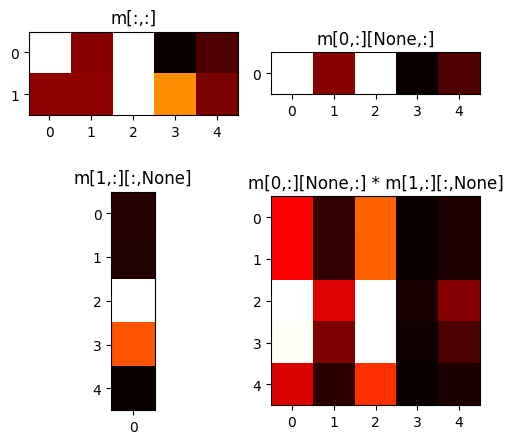
\includegraphics[width=0.5\textwidth]{assets/fig3.png}
    \caption{Outer product of two rows of a matrix}
\end{figure}
\end{exampleblock}

\subsection{Devices and types}

One of the big reasons to use pytorch instead of numpy is that pytorch can do computations on the GPU.  But because moving data on and off of a GPU device is more expensive than keeping it within the device, pytorch treats a Tensor's computing device as pseudo-type that requires explicit declaration and explicit conversion.  Here are some things to know about pytorch devices and types:

\begin{itemize}
    \item \textbf{Single precision CPU default}: by default a torch tensor will be stored on the CPU and will store single-precision 32-bit \texttt{torch.float} values 
    \item \textbf{Specifying data type}: to store a different data type such as integers, use the argument \texttt{dtype=torch.long} when you create the Tensor. As an example, \texttt{z = torch.zeros(10, dtype=torch.long)}. 
    \item \textbf{Specifying GPU}: to store the tensor on the GPU, specify \texttt{device='cuda'} when you make it, for example \texttt{identity\_matrix = torch.eye(5, device='cuda')}. Instead, \texttt{device='cpu'} indicates the default CPU storage.
    
    Even on a multi-GPU machine it is fine to pretend there is only one GPU. Setting the environment variable \texttt{CUDA\_VISIBLE\_DEVICES=3} before you start the program will set up the process to see GPU\#3 as the only GPU.  This is useful for debugging and for running multiple copies of the same program on the same machine.

    As an aside, in principle you could instead target one of many GPUs with \texttt{device='cuda:3'}, but if you want to use multiple GPUs for the same computation your best bet is to use a multiprocess utility class that manages data distribution between forked processes automatically, while each python process touches only one GPU.

    \item \textbf{Copying a tensor to a different device or type}: you cannot directly combine tensors that are on different devices (e.g. GPU vs CPU or different GPUs); this is similar to how most different data-type combinations are also prohibited. In both cases you will need to convert types and move devices explicitly to make tensors compatible before combining them. The \texttt{x.to(y.device)} or \texttt{x.to(y.type)} function can be used to do the conversion. 
    
    There are also commonly-used convenience synonyms \texttt{x.cpu()}, \texttt{x.cuda()}, \texttt{x.float()}, \texttt{x.long()}, etc. for making a copy of x with the specified device or type. There is a bit of cost, so move data only when needed. 

    \item \textbf{GPU rounding is nondeterministic}: computationally the GPU is not perfectly equivalent to the CPU. To speed parallelization, the GPU does not do associative operations such as summation in a deterministic sequential order. Since changing the order of summations can alter rounding behavior in fixed-precision arithmetic, GPU rounding can be different from CPU results an even nondeterministic. When the numerical algorithm is well-behaved, the difference should be small enough that you do not care, but you should know it is different. 
    \item \textbf{Float is faster}: all commodity GPU hardware is fast at single-precision 32-bit floating point math, about 20x CPU speed. Be aware that only expensive cards are fast at 64-bit double-precision math. If you change \texttt{torch.float} in the below example to \texttt{torch.double} on an Nvidia Titan or consumer card without hardware double-precision support, you will slow down to just-slightly-faster-than-CPU speeds. Similarly 16-bit \texttt{torch.half} or \texttt{torch.bfloat16} or other cool options will only be faster on newer hardware, and with these data types you need to take care that reduced precision is not damaging your results. 
    
    So \texttt{float} is the default and usually the best. 

    Also note that some operations (like linear algebra) are floating-point only and cannot be done on integers. 

    An example of some CPU versus GPU speed comparisons is below.

    \begin{exampleblock}[Speed comparison]
        \begin{codeblock}[language=python]
import torch, time
from matplotlib import pyplot as plt

# Here is a demonstration of moving data between GPU and CPU.
# We multiply a batch of vectors through a big linear opeation 10 times
r = torch.randn(1024, 1024, dtype=torch.float)
x = torch.randn(32768, 1024, dtype=r.dtype)
iterations = 10

def time_iterated_mm(x, matrix):
    start = time.time()
    result = 0
    for i in range(iterations):
        result += torch.mm(matrix, x.to(matrix.device).t())
    torch.cuda.synchronize()
    elapsed = time.time() - start
    return elapsed, result.cpu()

cpu_time, cpu_result = time_iterated_mm(x.cpu(), r.cpu())
print(f'time using the CPU alone: {cpu_time:.3g} seconds')

mixed_time, mixed_result = time_iterated_mm(x.cpu(), r.cuda())
print(f'time using GPU, moving data from CPU: {mixed_time:.3g} seconds')

pinned_time, pinned_result = time_iterated_mm(x.cpu().pin_memory(), r.cuda())
print(f'time using GPU on pinned CPU memory: {pinned_time:.3g} seconds')

gpu_time, gpu_result = time_iterated_mm(x.cuda(), r.cuda())
print(f'time using the GPU alone: {gpu_time:.3g} seconds')

plt.figure(figsize=(4,2), dpi=150)
plt.ylabel('iterations per sec')
plt.bar(['cpu', 'mixed', 'pinned', 'gpu'],
        [iterations/cpu_time,
            iterations/mixed_time,
            iterations/pinned_time,
            iterations/gpu_time])
plt.show()

print(f'Your GPU is {cpu_time / gpu_time:.3g}x faster than CPU'
        f' but only {cpu_time / mixed_time:.3g}x if data is repeatedly copied from the CPU')
print(f'When copying from pinned memory, speedup is {cpu_time / pinned_time:.3g}x')
print(f'Numerical differences between GPU and CPU: {(cpu_result - gpu_result).norm() / cpu_result.norm()}')
        \end{codeblock}
    \end{exampleblock}

    \begin{figure}[H]
        \centering
        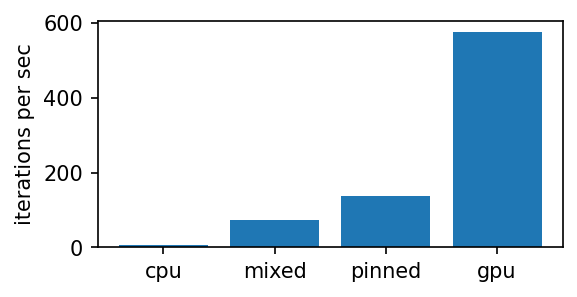
\includegraphics[width=0.5\textwidth]{assets/fig4.png}
        \caption{Speed comparison between CPU and GPU}
    \end{figure}
\end{itemize}

\subsection{Performance tips}

\textbf{GPU operations are async}. When pytorch operates on GPU tensors, the python code does not wait for computations to complete. Sp GPU calculations get queued up, and they will be done as quickly as possible in the background while your python is free to work on other things like loading the next batch of training data.

\textbf{Moving data to cpu waits for computations.} You do not need to worry about the GPU asynchrony, because as soon as you actually ask to look at the data, e.g., when you move GPU data to CPU (or print it or save it), pytorch will block and wait for the GPU operations to finish computing what you need before proceeding. The call seen above to \texttt{torch.cuda.synchronize()} flushes the GPU queue without requesting the data, but you will not need to do this unless you are doing performance timing.

\textbf{Pinned memory transfers are async and faster.} Copying data from CPU to GPU can be sped up if the CPU data is put in pinned memory (i.e., at a fixed non-swappable block of RAM).  Therefore when data loaders gather together lots of CPU data that is destined for the GPU, they should be configured to stream their results into pinned memory. See the performance comparison above.

\subsection{PyTorch Tensor dimension-ordering conventions}

\textbf{Multidimensional data convension.} As soon as you have more than one dimension, you need to decide how to order the axes.  To reduce confusion, most data processing follows the same global convention. In particular, much image-related data in pytorch is four dimensional, and the dimensions are ordered like this: \texttt{data[batch\_index, channel\_index, y\_position, x\_position]}, that is:
\begin{itemize}
    \item Dimension 0 is used to index separate images within a batch.
    \item Dimension 1 indexes channels within an image representation (e.g., 0,1,2 = R,G,B, or more dims for more channels).
    \item Dimension 2 (if present) indexes the row position (y-value, starting from the top)
    \item Dimension 3 (if present) indexes the column position (x-value, starting from the left)
\end{itemize}

There a way to remember this ordering: adjacent entries that vary only in the last dimensions are stored physically closer in RAM; since they are often combined with each other, this could help with locality, whereas the first (batch) dimension usually just groups separate independent data points which are not combined much, so they do not need to be physically close.

Stream-oriented data without grid geometry will drop the last dimensions, and 3d grid data will be 5-dimensional, adding a depth z before y.  This same 4d-axis ordering convention is also seen in caffe and tensorflow.

Separate tensors can be put together into a single batch tensor using \texttt{torch.cat([a, b, c])} or \texttt{torch.stack([a, b, b])}.

\textbf{Multidimensional linear operation convention.} When storing matrix weights or a convolution weights, linear algebra conventions are followed:
\begin{itemize}
    \item Dimension 0 (number of rows) matches the output channel dimension
    \item Dimension 1 (number of columns) matches the input channel dimension
    \item Dimension 2 (if present) is the convolutional kernel y-dimension
    \item Dimension 3 (if present) is the convolutional kernel x-dimension
\end{itemize}

Since this convention assumes channels are arranged in different rows whereas the data convention puts different batch items in different rows, some axis transposition is often needed before applying linear algebra to the data.

\textbf{Permute and view reshape an array without moving memory.} The \texttt{permute} and \texttt{view} methods are useful for rearranging, flattening and unflattening axes. \texttt{x.permute(1,0,2,3).view(x.shape[1],-1)}. They just alter the view of the block of numbers in memory without moving any of the numbers around, so they are fast.

\textbf{Reshaping sometimes needs copying.} Some sequences of axis permutations and flattenings cannot be done without copying the data into the new order in memory; the \texttt{x.contiguous()} method copies the data iinto the natural order given by the current view; also \texttt{x.reshape()} is similar to \texttt{view} but will makea copy if necessary so you do not need to think about it.

\subsection{Einsum notation}

Matrix multiplication can be generalized to tensors of arbitrary number of dimensions, but keeping tensor dimensions straight can be confusing. The solution to this is \href{https://en.wikipedia.org/wiki/Einstein_notation}{Einstein notation}: assign letter variables to each axis of the input tensors, and then explicitly write down which axes end up in the output tensor.  For example, an outer product might be written as \texttt{i, j -> ij}, whereas matrix multiplication could be \texttt{ij, jk -> ik}.

Einstein notation is a topic of active development and programming language design: \href{https://openreview.net/pdf?id=oapKSVM2bcj}{here is a recent paper on the history and future of Einstein APIs.}

In PyTorch, Einstein notation is available as \texttt{einsum}. Here is how ordinary matrix multiplication looks as einsum:

\begin{exampleblock}[Einsum]
    \begin{codeblock}[language=python]
A = torch.randn(2,5)
B = torch.randn(5,3)

# Uncomment to see ordinary matrix multiplication
# print(torch.mm(A, B))

# Ordinary matrix multiplication written as an einsum
print(torch.einsum('ij, jk -> ik', A, B))
    \end{codeblock}
\end{exampleblock}





\newpage
\section{Autograd}

If you flag a torch Tensor with the attribute \texttt{x.requires\_grad=True}, then PyTorch will automatically keep track the computational history of all tensors that are derived from \texttt{x}. This allows PyTorch to figure out derivatives of any scalar result with regard to changes in the components of x. 

\begin{figure}[H]
    \centering
    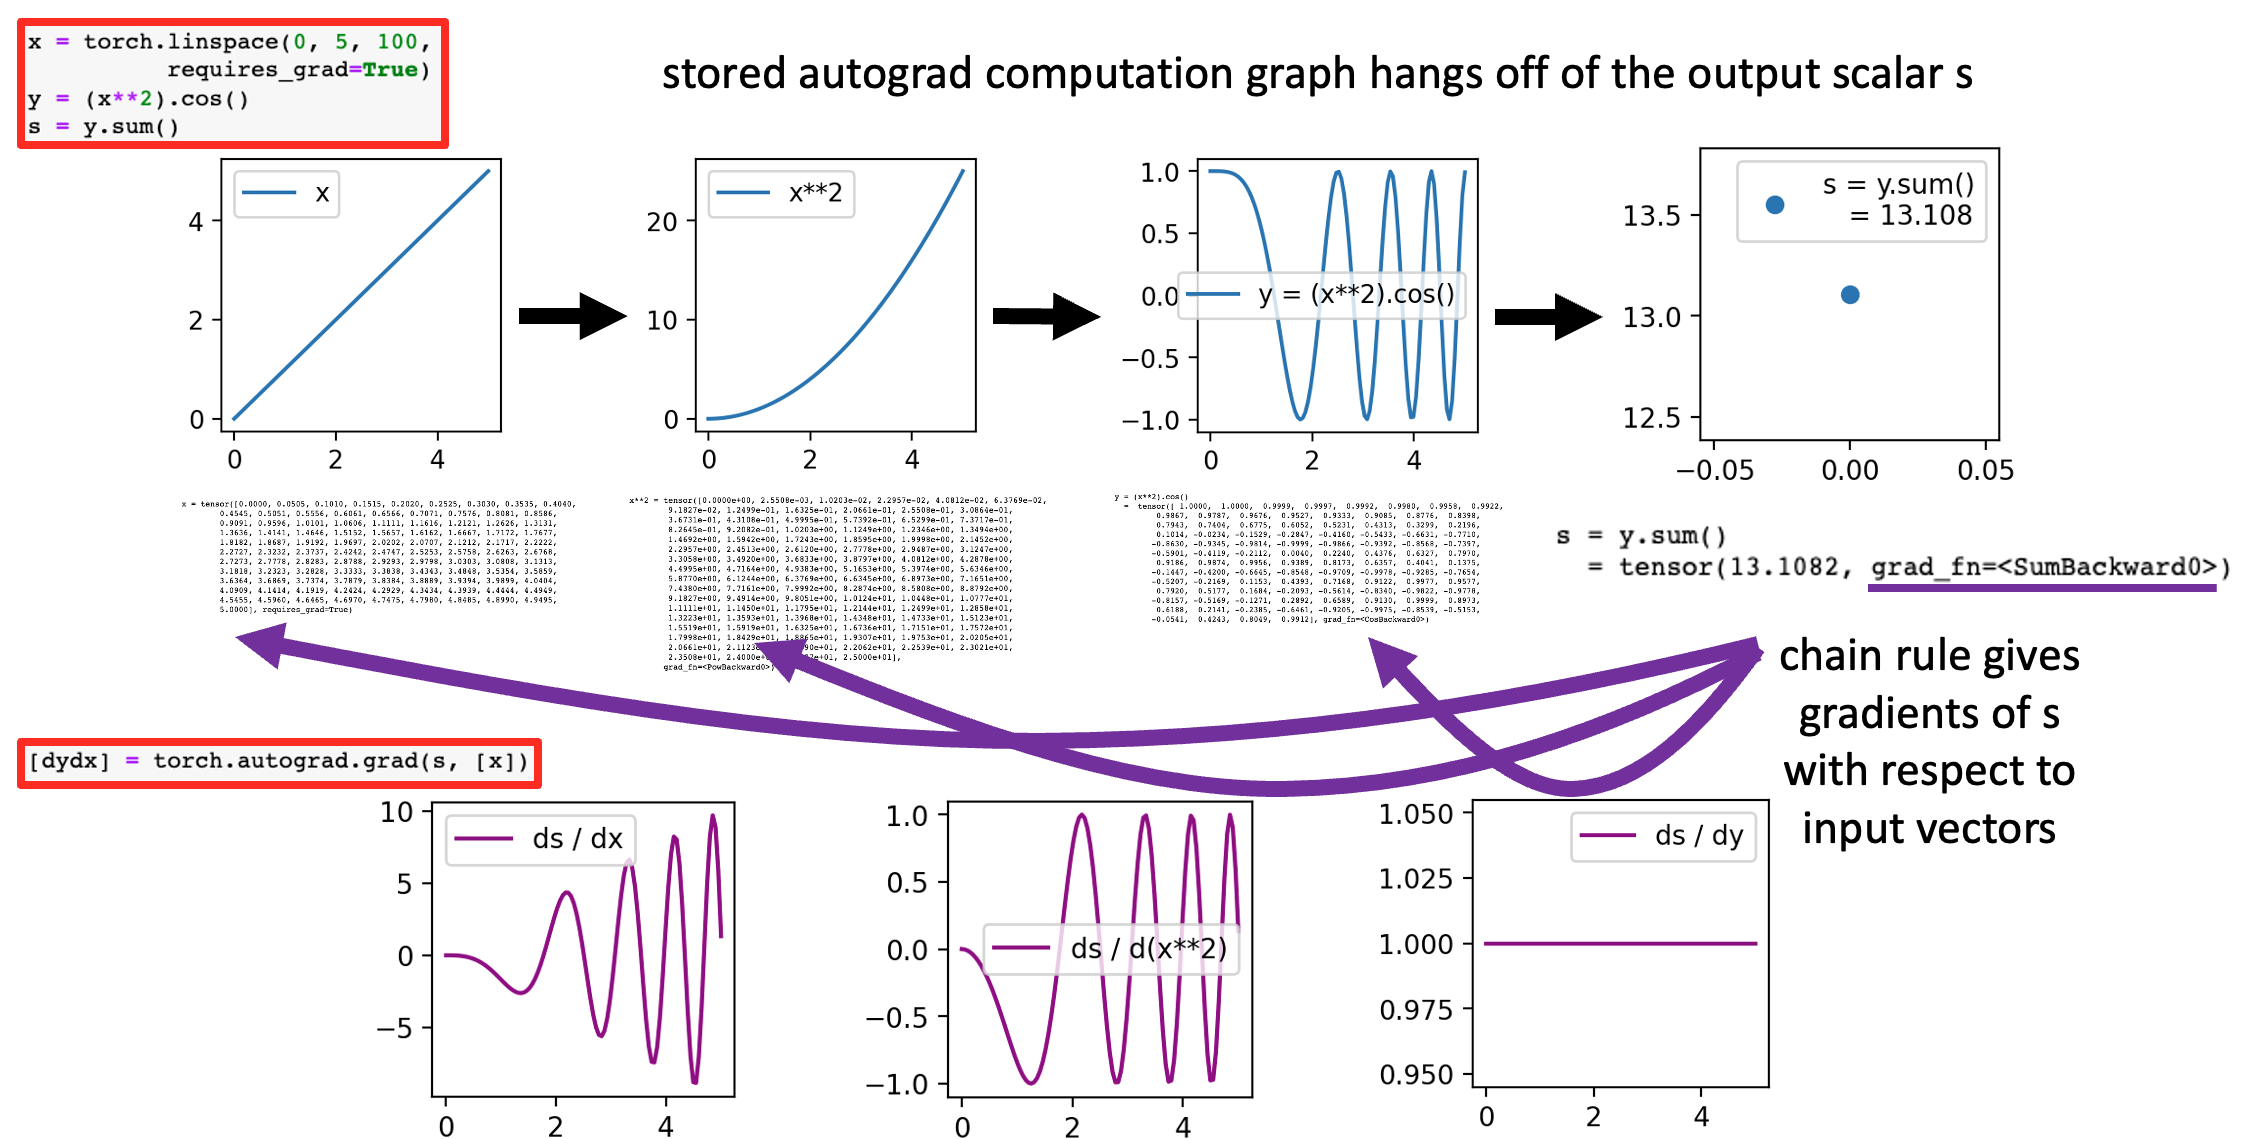
\includegraphics[width=0.9\textwidth]{assets/autograd-graph.png}
    \caption{Computational graph}
\end{figure}

The function \texttt{torch.autograd.grad(output\_scalar, [list of input\_tensors])} will return a list of the derivatives of the output scalar with respect to each of the input tensors. It computes \texttt{d(output\_scalar)/d(input\_tensor)} for each input tensor component in the list. For it to work, the input tensors and output must be part of the same \texttt{requires\_grad = True} computation. 

In the example below,, \texttt{x} is explicitly marked \texttt{requires\_grad = True}, so \texttt{y.sum()}, which is derived from x, automatically comes along with the computation history, and can be differentiated. 

\begin{exampleblock}[Autograd]
    \begin{codeblock}[language=python]
import torch
from matplotlib import pyplot as plt

x = torch.linspace(0, 5, 100,
            requires_grad=True)
y = (x**2).cos()
s = y.sum()
[dydx] = torch.autograd.grad(s, [x])

plt.plot(x.detach(), y.detach(), label='y')
plt.plot(x.detach(), dydx, label='dy/dx')
plt.legend()
plt.show()
    \end{codeblock}
\end{exampleblock}

\begin{figure}[H]
    \centering
    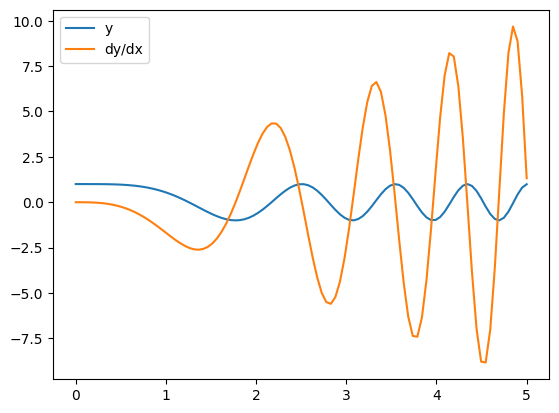
\includegraphics[width=0.5\textwidth]{assets/fig5.png}
    \caption{Derivative of $y = \cos(x^2)$}
\end{figure}

\begin{observationblock}[Example above]
    Note that in the above example, because the components of the vector space are independent of each other, we happen to have \texttt{dy[j] / dx[i] == 0} when \texttt{j != i}, so that \texttt{d(y.sum())/dx[i] = dy[i]/dx[i]}. That means computing a single gradient vector of the sum \texttt{s} is equivalent to computing elementwise derivatives \texttt{dy/dx}. 
\end{observationblock}

Every tensor that depends on \texttt{x} will be \texttt{requires\_grad = True} and connected to the complete computation history. But if you were to convert a tensor to a regular python number, PyTorch would not be able to see the calculations and would not be able to compute gradients on it. 

To avoid programming mistakes where some computation invisibly goes through a non-PyTorch number that cannot be tracked, PyTorch disables requires-grad tensors from being converted to untrackable numbers. You need to explicitly call \texttt{x.detach()} or \texttt{y.detach()} first, to explicitly say that you want an untracked reference, before plotting the data or using it as non-PyTorch numbers. 

\subsection{Backpropagation and In-Place gradients}

In a typical neural network we will not just be getting gradients with regard to one input like \texttt{x} above, but with regard to a list of dozens or hundreds of tensor parameters that have all been marked with \texttt{requires\_grad = True}. It can be inconvenient to keep track of which gradient outputs go with which original tensor input. But since the gradients have exactly the same shape as the inputs, it is natural to store computed gradients in-place on the tensors themselves. 

To simplify this common operation, PyTorch provides the \texttt{.backward()} methods, which computes the gradients of y with respect to every tracked dependency, and stores the results in the field \texttt{x.grad} for every input vector \texttt{x} that was marked as \texttt{requires\_grad = True}. 

\begin{codeblock}[language=python]
x = torch.linspace(0, 5, 100, requires_grad=True)
y = (x**2).cos()
y.sum().backward()   # populates the grad attribute below.
print(x.grad)

plt.plot(x.detach(), y.detach(), label='y')
plt.plot(x.detach(), x.grad, label='dy/dx')
plt.legend()
plt.show()
\end{codeblock}

\subsection{Accumulating and zeroing gradients}

If you find that your data batches are too large to get gradients of the whole thing, then it is usually possible to split the batches into smaller pieces and add the gradients. Because gradient accumulation is a common pattern, if you call \texttt{.backward()} when parameters \texttt{x.grad} already exists, it is not an error. The new gradient will be added to the old one. 

That means that you need to set any previous value of \texttt{x.grad} to zero before running \texttt{backward()}, or else the new gradient will be added to the old one. Optimizers have a utility \texttt{optim.zero\_grad()} to do this to all the optimized parameters at once. 

\subsection{Saving memory on inference}

Normally, all the parameters of a neural network are set to \texttt{requires\_grad = True} by default, so they are ready to be trained. But that means that whenever you run a network you will get output which is also requires-grad, and it will be attached to a long computation history that consumes a lot of precious GPU memory. 

To avoid all this expense when you have no intention of training the network, you could go through all the network parameters to set \texttt{requires\_grad = False}.

Another way to avoid the computation history is to enclose the entire computation within a \texttt{with torch.no\_grad():} block. This will suppress all the autograd mechanics (which means \texttt{.backward()} will not work) and will save memory.

Note that this is different from the role of \texttt{net.eval()} which puts the network in inference mode computationally (batchnorm, dropout, and other operations behave differently in training and inference); \texttt{net.eval()} does not have any effect on \texttt{requires\_grad}.

Moreover:
\begin{itemize}
    \item Normally gradients with respect to intermediate values are not stored in \texttt{.grad}, but you can ask for intermediate gradients oìto be stored using \texttt{v.retain\_grad()}.
    \item If you want higher-order derivatives, then you want PyTorch to build the computation graph when is computing the gradient itself, so this graph can be differentiated again. To do this, use the \texttt{create\_graph = True} option on the \texttt{grad} or \texttt{backward} methods. 
    \item Usually you only need to call \texttt{y.backward()} once per computation tree, and PyTorch will not let you call it again. To save memory, PyTorch will have deallocated the computation graph after you have computed a single gradient. But if you need more than one gradient, you can use \texttt{retain\_graph = True}.
\end{itemize}


\section{PyTorch Optimizers}

Optimizers have a simple job: given gradients of an objective with respect to a set of input parameters, adjust the parameters reduce te objective. They o this by modifying each parameter by a small amount in the direction given by the gradient. 

\begin{codeblock}[language=python]
#@title Run this cell to setup visualization...
# This cell defines plot_progress() which plots an optimization trace.

import matplotlib
from matplotlib import pyplot as plt

def plot_progress(bowl, track, losses):
    # Draw the contours of the objective function, and x, and y
    fig, (ax1, ax2) = plt.subplots(1,2, figsize=(12, 5))
    for size in torch.linspace(0.1, 1.0, 10):
        angle = torch.linspace(0, 6.3, 100)
        circle = torch.stack([angle.sin(), angle.cos()])
        ellipse = torch.mm(torch.inverse(bowl), circle) * size
        ax1.plot(ellipse[0,:], ellipse[1,:], color='skyblue')
    track = torch.stack(track).t()
    ax1.set_title('progress of x')
    ax1.plot(track[0,:], track[1,:], marker='o')
    ax1.set_ylim(-1, 1)
    ax1.set_xlim(-1.6, 1.6)
    ax1.set_ylabel('x[1]')
    ax1.set_xlabel('x[0]')
    ax2.set_title('progress of y')
    ax2.xaxis.set_major_locator(matplotlib.ticker.MaxNLocator(integer=True))
    ax2.plot(range(len(losses)), losses, marker='o')
    ax2.set_ylabel('objective')
    ax2.set_xlabel('iteration')
    fig.show()

from IPython.display import HTML
HTML('''<script>function toggle_code(){$('.rendered.selected div.input').toggle().find('textarea').focus();} $(toggle_code())</script>
<a href="javascript:toggle_code()">Toggle</a> the code for plot_progress.''')
\end{codeblock}

\subsection{Gradient Descent just abstracts the gradient}

You can apply gradient descent by hand easily by just using \texttt{loss.backward()} to compute the gradient of the loss with respect to every possible parameter \texttt{x}, and then apply \texttt{x -= learning\_rate * x.grad} to nudge \texttt{x} in the gradient direction that makes the loss smaller. 

Here is an example of gradient descent on a simple bowl-shaped objective function.

\begin{exampleblock}[Gradient Descent]
    \begin{codeblock}[language=python]
import torch

x_init = torch.randn(2)
x = x_init.clone()

bowl = torch.tensor([[ 0.4410, -1.0317], [-0.2844, -0.1035]])
track, losses = [], []

for iter in range(21):
    x.requires_grad = True
    loss = torch.mm(bowl, x[:,None]).norm()
    loss.backward()
    with torch.no_grad():
        x = x - 0.1 * x.grad
    track.append(x.detach().clone())
    losses.append(loss.detach())
    
plot_progress(bowl, track, losses)
    \end{codeblock}
\end{exampleblock}

\begin{figure}[H]
    \centering
    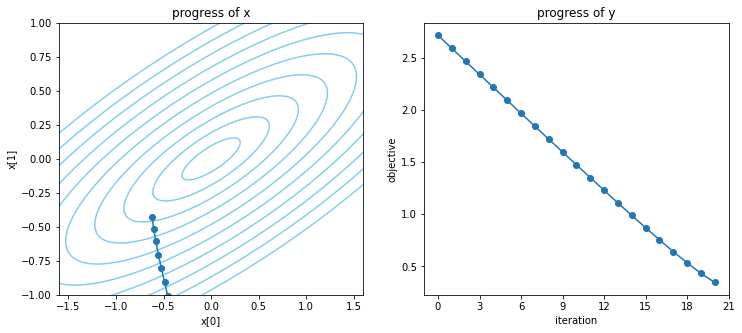
\includegraphics[width=0.7\textwidth]{assets/fig6.png}
    \caption{Gradient Descent}
\end{figure}

\subsection{Built-in optimization algorithms}

PyTorch includes several optimization algorithms. 

The actual optimization algorithms employ a number of techniques to make the process faster and more robust as repeated steps are taken, by trying to adapt to the shape of the objective surface as it is explored. The simplest method is SGD-with-momentum, which is implemented in PyTorch as \texttt{pytorch.optim.SGD}.

To use SGD, you need to calculate your objective and fill in gradients on all the parameters before it can take a step. 
\begin{enumerate}
    \item Set your parameters (x in this case) to \texttt{x.requires\_grad = True} so autograd tracks them
    \item Create the optimizer and tell it about the parameters to adjust ([x] here)
    \item In a loop, compute your objective, then call \texttt{loss.backward()} to fill in \texttt{x.grad} and then \texttt{optimizer.step()} to adjust x accordingly
\end{enumerate}

Notice that we use \texttt{optimizer.zero\_grad()} each time to set x.grad to zero before recomputing gradients; if we do not do this, then the new gradient will be added to the old one. 

\begin{exampleblock}[SGD]
    \begin{codeblock}[language=python]
import torch

x = x_init.clone()
x.requires_grad = True
optimizer = torch.optim.SGD([x], lr=0.1, momentum=0.5)

bowl = torch.tensor([[ 0.4410, -1.0317], [-0.2844, -0.1035]])
track, losses = [], []

for iter in range(21):
    loss = torch.mm(bowl, x[:,None]).norm()
    optimizer.zero_grad()
    loss.backward()
    optimizer.step()
    track.append(x.detach().clone())
    losses.append(loss.detach())
    
plot_progress(bowl, track, losses)
    \end{codeblock}
\end{exampleblock}

\begin{figure}[H]
    \centering
    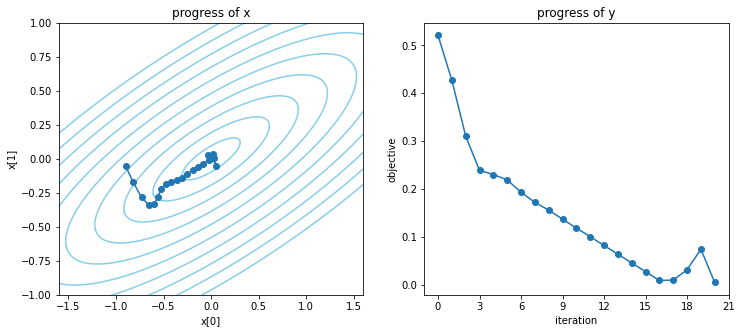
\includegraphics[width=0.7\textwidth]{assets/fig7.png}
    \caption{SGD}
\end{figure}

Other optimizers are similar. Adam is a popular adaptive method that does well without much tuning, and can be dropped in to replace plain SGD.

Some other fancy optimizers, such as LBFGS, need to be given an objective function that they can call repeatedly to probe gradients themselves. 

\begin{exampleblock}[Adam]
    \begin{codeblock}[language=python]
# The code below uses Adam
x = x_init.clone()
x.requires_grad = True
optimizer = torch.optim.Adam([x], lr=0.1)

track, losses = [], []

for iter in range(21):
    loss = torch.mm(bowl, x[:,None]).norm()
    optimizer.zero_grad()
    loss.backward()
    optimizer.step()
    track.append(x.detach().clone())
    losses.append(loss.detach())
    
plot_progress(bowl, track, losses)
    \end{codeblock}
\end{exampleblock}

\begin{figure}[H]
    \centering
    
\includegraphics[width=0.7\textwidth]{assets/fig8.png}
    \caption{Adam}
\end{figure}

\subsection{Other tricks}

\begin{itemize}
    \item \textbf{Learning rate schedules}: one of the simplest and most effective ways to improve training is to adjust the learning rate, decreasing it during training.   There are many differerent strategies for scheduling learning rates, and pytorch comes with a set of \texttt{torch.optim.lr\_scheduler} classes to make it easy to drop in a variety of methods.
    \item \textbf{Mutliple optimizers}: Sometimes you want to optimize more than one objective.  The ordinary solution to this is to make an single overall objective as a (weighted) sum of all the objectives.  However, sometimes you want to apply one objective to some parameters and a different objective to a different set of parameters.  This occurs, for example in \textit{adversarial training} such as in GANs, where two networks are learning to play against each other.  In this case you can use multiple different optimizers, one for each opposing objective.
\end{itemize}


\newpage
\section{NN modules}

PyTorch uses the \texttt{torch.nn.Module} class to represent a neural network. A \texttt{Module} is a callable function that can be:
\begin{itemize}
    \item \textbf{Parametrized} by trainable \texttt{Parameter} tensors that the module can list out 
    \item \textbf{Composed} out of children \texttt{Module}s that contribute parameters
    \item \textbf{Saved and Loaded} by listing named parameters and other attribute buffers
\end{itemize}

PyTorch comes with several built-in elementary network modules like a generic single-layer \texttt{Linear} network, or a generic \texttt{Sequential} composition of other networks, but of course you can write your own \texttt{Module} subclasses by just defining \texttt{Parameter} attributes and using them to implement a computation. 

To see how every \texttt{Module} manages its own portion of responsibilities of all the network duties above, we first look at how to use the built-in \texttt{Linear} and \texttt{Sequential} modules. 

\subsection*{Using \texttt{torch.nn.Linear as NN}}

The linear layer is not just a good starting example: it is the fundamental workhorse of all neural networks, so as simple as it is, it is worth examining carefully. 

\texttt{torch.nn.Linear} implements the function \textbf{$y = Ax + b$}, which takes m-dimensional input \texttt{x} and produces n-dimensional output \texttt{y}, by multiplying by the $n\times n$ matrix \texttt{A} (whose specific values are called the \textbf{weights}) and adding n-dimensional vector \texttt{b} (whose values are called the \textbf{bias}). We can make a Linear network with 3D input and 2D output just like the following:


\begin{codeblock}[language=python]
import torch
net = torch.nn.Linear(3, 2)
print(net)
\end{codeblock}

Like any Module, our little network can be run as a function. As expected, when we give it 3D vectors as input, we get a 2D vector as output. 

\begin{codeblock}[language=python]
    net(torch.tensor([[1.0, 0.0, 0.0]]))
    # tensor([[ 0.0000, -0.0734]], grad_fn=<AddmmBackward>)
\end{codeblock}

\begin{observationblock}[Linear network]
    Notice the double nesting in the vector data above. This is needed because out \texttt{Linear} network is slightly different from a plain matrix-vector multiplication. By convention, PyTorch Modules are set up to process data in batches, so to give it a single 3D vector, instead of passing just a vector, we have passed it a singleton batch containing one vector. 
    \begin{codeblock}[language=python]
x_batch = torch.tensor([
    [1.0, 0. , 0. ],
    [0. , 1.0, 0. ],
    [0. , 0. , 1.0],
    [0. , 0. , 0. ],
])
#tensor([[-0.4530,  0.6047],
#       [-0.3436, -0.0084],
#       [-0.0957,  0.2989],
#       [-0.1118,  0.0888]], grad_fn=<AddmmBackward0>)
    \end{codeblock}
\end{observationblock}

By default, the weights and biases of the \texttt{Linear} network are initialized randomly.  You can see the values of the weights and biases by looking at the \texttt{.weight} and \texttt{.bias} attributes of the network.
\begin{codeblock}[language=python]
print(net.weight)
print(net.bias)
\end{codeblock}

Above you can see that bothe the weight and the bias are trainable parameters, because they both have the \texttt{Parameter} type. The tensors also both marked as \texttt{requires\_grad = True}, which means that they are marked to participate in autograd and optimization for training. 

These are the only two trainable parameters of the network. To check this, we can list all the parameters by name, with \texttt{net.named\_parameters()}.

\begin{codeblock}[language=python]
for name, param in net.named_parameters():
print(f'{name} = {param}\n')

#weight = Parameter containing:
#tensor([[-0.3413, -0.2319,  0.0160],
#        [ 0.5159, -0.0972,  0.2101]], requires_grad=True)

#bias = Parameter containing:
#tensor([-0.1118,  0.0888], requires_grad=True)
\end{codeblock}

A module can also be saved by saving its state dictionary, which includes all the parameters and buffers. \texttt{net.state\_dict()} is similar to \texttt{net.named\_parameters()} but it returns a detached reference to the data (i.e.,  texttt{requires\_grad = False}) so the data can be saved directly. Also, for more complicated modules, \texttt{state\_dict()} may include other non-trainable attributes that are needed to save the network's state. 

\begin{codeblock}[language=python]
for k, v in net.state_dict().items():
    print(f'{k}: {v.type()}{tuple(v.shape)}')

import os
os.makedirs('checkpoints', exist_ok=True)
torch.save(net.state_dict(), 'checkpoints/linear.pth')

# weight: torch.FloatTensor(2, 3)
# bias: torch.FloatTensor(2,)
\end{codeblock}

PyTorch also comes with convenient \texttt{torch.save} and \texttt{torch.load} functions for saving state dicts to files. 

\begin{codeblock}[language=python]
net.load_state_dict(torch.load('checkpoints/linear.pth'))

# <All keys matched successfully>
\end{codeblock}

\subsection{Training Example: Optimizing a Linear Layer}

To train a network we need to come up with a score for how close we are to the goal. This scalar number is called the \textbf{objective} or the \textbf{loss}. 

As an example, suppose we would like this network to always output \texttt{[1, 1]} regardless of input. Then a reasonable loss would be the mean suqared distance to \texttt{[1, 1]}, computed like this:
\begin{codeblock}[language=python]
y_batch = net(x_batch)
loss = ((y_batch - torch.tensor([[1.0, 1.0]])) ** 2).sum(1).mean()
print(f'loss is {loss}')
\end{codeblock}

We can use autograd get gradients to see how small changes in every parameter would impact the loss. 

\begin{codeblock}[language=python]
loss.backward()
print(net.weight.grad)
print(net.bias.grad)
# tensor([[ 0.0000,  0.0000, -0.0000],
#        [ 0.0000,  0.0000, -0.0000]])
# tensor([0.0000, 0.0000])
# Note that the gradients are all zero, because the output is already at the target value.
# If we change the target to [0, 0], then the gradients are non-zero.
loss = ((y_batch - torch.tensor([[0.0, 0.0]])) ** 2).sum(1).mean()
loss.backward()
print(net.weight.grad)
# tensor([[ 0.0000,  0.0000, -0.0000],
#        [ 0.0000,  0.0000, -0.0000]])
print(net.bias.grad)
# tensor([-0.0000, -0.0000])
\end{codeblock}

\textbf{Simple gradient descent can be done directly}. To improve our layer, we can use simple gradient descent with a learning rate of 0.01. That is, we can adjust each parameter by subtracting 0.01 times the gradient. If we do this repeatedly, we should get closer to our objective. 

Any time we directly update the network parameters, we need to temporarily disable the autograd machinery using \texttt{with torch.no\_grad()}.

\begin{codeblock}[language=python]
net = torch.nn.Linear(3, 2)
log = []
for _ in range(10000):
    y_batch = net(x_batch)
    loss = ((y_batch - torch.tensor([[1.0, 1.0]])) ** 2).sum(1).mean()
    log.append(loss.item())
    net.zero_grad()
    loss.backward()
    with torch.no_grad():
        for p in net.parameters():
            p[...] -= 0.01 * p.grad
print(f'weight is {net.weight}\n')
print(f'bias is {net.bias}\n')

%matplotlib inline
import matplotlib.pyplot as plt
plt.ylabel('loss')
plt.xlabel('iteration')
plt.plot(log)
plt.show()

#weight is Parameter containing:
#tensor([[7.5908e-06, 7.5909e-06, 7.5911e-06],
#        [1.4001e-05, 1.4001e-05, 1.4001e-05]], requires_grad=True)
#
#bias is Parameter containing:
#tensor([1.0000, 1.0000], requires_grad=True)
\end{codeblock}

\begin{figure}[H]
    \centering
    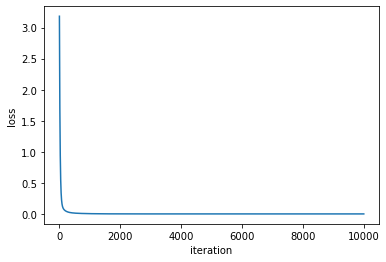
\includegraphics[width=0.5\textwidth]{assets/fig9.png}
    \caption{Loss over iterations}
\end{figure}

\subsection{Using \texttt{torch.nn.Sequential} to compose networks}

Unlike \texttt{Linear}, most networks are made by composing many smaller networks. The simplest way to do this is chain networks together end-to-end, connecting each outpu to the next input. For example, we can simply compose \texttt{Linear} layers. 

\textbf{Defining Multilayer Perceptron}. Of course, to get something more interesting than another linear function, we need to do something nonlinear between the linear steps. If we add a nonlinearity between each step (for example, if we clamp negative numbers to zero - an operation called \textbf{ReLU}), then we can get a \textbf{Multilayer Perceptron}, which is known to be a universal function approximator, i.e., a family of piecewise-linear functions that can approximate any function. 

Here is how we can express the network as a nested set of Sequentials:

\begin{codeblock}[language=python]
from collections import OrderedDict
from torch.nn import Linear, ReLU, Sequential

mlp = torch.nn.Sequential(OrderedDict([
('layer1', Sequential(Linear(2, 20), ReLU())),
('layer2', Sequential(Linear(20, 20), ReLU())),
('layer3', Sequential(Linear(20, 2)))
]))

print(mlp)

#Sequential(
#  (layer1): Sequential(
#    (0): Linear(in_features=2, out_features=20, bias=True)
#    (1): ReLU()
#  )
#  (layer2): Sequential(
#    (0): Linear(in_features=20, out_features=20, bias=True)
#    (1): ReLU()
#  )
#  (layer3): Sequential(
#    (0): Linear(in_features=20, out_features=2, bias=True)
#  )
#)
\end{codeblock}

In the above, we have nested two levels of Sequentials. In the outermost level, we have defined and named three layers. 

Then each layer is itself a Sequential that executes a parametrized \texttt{Linear} operation followed by a \texttt{ReLU} nonlinear clamping operation. We have not bothered to name each of the innermost steps, so the Sequential just automatically numbers them. 

\textbf{Every submodule has a fully qualified name}. We can het a full recursive list of submodules by listing \texttt{net.named\_modules()}. 

\begin{codeblock}[language=python]
for n, c in mlp.named_modules():
print(f'{n or "The whole network"} is a {type(c).__name__}')

#The whole network is a Sequential
#layer1 is a Sequential
#layer1.0 is a Linear
#layer1.1 is a ReLU
#layer2 is a Sequential
#layer2.0 is a Linear
#layer2.1 is a ReLU
#layer3 is a Sequential
#layer3.0 is a Linear

\end{codeblock}

\textbf{A module's parameters include all its child module parameters}. We can see this by listing all the parameters by name. 

\begin{codeblock}[language=python]
for name, param in mlp.named_parameters():
print(f'{name} has shape {tuple(param.shape)}')

#layer1.0.weight has shape (20, 2)
#layer1.0.bias has shape (20,)
#layer2.0.weight has shape (20, 20)
#layer2.0.bias has shape (20,)
#layer3.0.weight has shape (2, 20)
#layer3.0.bias has shape (2,)
\end{codeblock}

There are now six parameters: a weight and a bias for each of the three \texttt{Linear} layers. 

\textbf{Training a Classifier}. This slightly more complicated network can now represent a more general class of functions. As an example, we can use this architecture to learn to compute a classifier function. 

Suppose we want to classify points on a plane as either above a sine-wave (class 1) or below a sine-wave (class 0). Here is the ordinary training loop to train our MLP to do it, using the Adam optimizer:

\begin{codeblock}[language=python]
from torch.nn.functional import cross_entropy

def classify_target(x, y):
    return (y > (x * 3).sin()).long()

mlp.cuda()
optimizer = Adam(mlp.parameters(), lr=0.01)
for iteration in range(1024):
    in_batch = torch.randn(10000, 2, device='cuda')
    target_batch = classify_target(in_batch[:,0], in_batch[:,1])
    out_batch = mlp(in_batch)
    loss = cross_entropy(out_batch, target_batch)
    if iteration > 0:
        mlp.zero_grad()
        loss.backward()
        optimizer.step()
    if iteration == 2 ** iteration.bit_length() - 1:
        pred_batch = out_batch.max(1)[1]
        accuracy = (pred_batch == target_batch).float().sum() / len(in_batch)
        print(f'Iteration {iteration} accuracy: {accuracy}')
        visualize_net(mlp, classify_target)
\end{codeblock}

\begin{figure}[H]
    \centering
    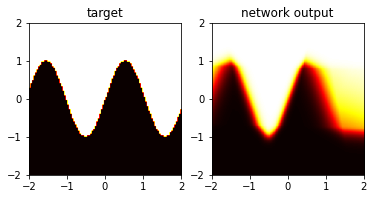
\includegraphics[width=0.5\textwidth]{assets/fig10.png}
    \caption{Classifier accuracy}
\end{figure}

\subsection{Defining \texttt{forward} to create custom networks}

Sometimes you will want to hook up network components in a more complicated way than just a sequential operation of predefined components. 

For example, \href{https://arxiv.org/abs/1512.03385}{ResNet} is built on the observation that learning can work much better if, instead of learning an arbitrary linear operation, we learn perturbations of the identity. I.e., have a layer learn to compute a small residual instead of the whole total answer. 

To apply the residual trick in our little three-layer network, we cannot just use an overall \texttt{Sequential}: instead we will define the operation by writing our own \texttt{forward} function. It looks like this:

\begin{codeblock}[language=python]
class MyNetwork(torch.nn.Module):
def __init__(self):
    super().__init__()
    self.layer1 = Sequential(Linear(2, 20), ReLU())
    self.residual_layer2 = Sequential(Linear(20, 20), ReLU())
    self.layer3 = Linear(20, 2)
    
def forward(self, x):
    x = self.layer1(x)
    x = x + self.residual_layer2(x)
    x = self.layer3(x)
    return x

res_mlp = MyNetwork()
print(res_mlp)

# Exercise left to you: try training res_mlp just like we trained mlp above.


#MyNetwork(
#  (layer1): Sequential(
#    (0): Linear(in_features=2, out_features=20, bias=True)
#    (1): ReLU()
#  )
#  (residual_layer2): Sequential(
#    (0): Linear(in_features=20, out_features=20, bias=True)
#    (1): ReLU()
#  )
#  (layer3): Linear(in_features=20, out_features=2, bias=True)
#)
 \end{codeblock}
 
 Training the network above can be done exactly the same way as training our previous \texttt{Sequential} mlp. Try copying+pasting the training code and adapting it to this new network. 

 \subsection{Other \texttt{Module} tricks}

 \begin{itemize}
    \item \texttt{torch.nn.Parameter} wraps trainable parameters. In the \texttt{\_\_init\_\_()} method, you can define more tensors as parameters to be optimized, by wrapping parameter tensors with a \texttt{torch.nn.Parameter} before setting the attribute. See the \href{https://github.com/pytorch/pytorch/blob/main/torch/nn/modules/linear.py#L74-L78}{pytorch Linear source code} to see an example. 
    \item \texttt{module.training} allows special behavior during training. Some modules behave differently at training time than at inference time. For example a \href{https://jmlr.org/papers/volume15/srivastava14a/srivastava14a.pdf}{Dropout} layer will drop half the channels and amplify the other half randomly during training, but at inference, for better performance, it will include all the channels. To support this sort of trick, there is a \texttt{module.train()} method to put a module (recursively) into training mode and a \texttt{module.eval()} to put it into inference mode. The \texttt{module.training} boolean tells which mode is current. 
    \item \textbf{buffers} can be learned without the optimizer. Not every attribute of a module needs to be trainable by the optimizer. Some attributes can be learned in a different way, for example by observing and averaging statistics observed during training time. The most famous example of this is the \href{https://arxiv.org/abs/1502.03167}{Batchnorm} layer, which observes mean and variance during training, and accumulates statistics to enforces zero mean and unit variance.
    \item \textbf{Predefined model architecture} are available; for example \texttt{torchvision.models.resnet18(num\_classes=100)} will create a ResNet-18 classifier model, configured to do a 100-way classification of images. 
 \end{itemize}



 \section{Datasets and Dataloaders in PyTorch}

 \begin{codeblock}[language=python]
# To save time, start this download first, before reading through the examples.
import torch, torchvision, os
if not os.path.isfile('datasets/miniplaces/train/yard/00001000.jpg'):
    torchvision.datasets.utils.download_and_extract_archive(
        'http://dissect.csail.mit.edu/datasets/miniplaces.zip',
        'datasets', md5='bfabeb497c7eca01c74cd8441a9ac108')
\end{codeblock}

Data sets can be thought of as big arrays of data. If the data set is small enough (e.g. MNIST, which has 60,000 28x28 grayscale images), a dataset can be literally represented as an array - or more precisely, as a single PyTorch tensor. With one number per pixel, MNIST takes about 200MB of RAM, which fits comfortably into a modern computer.

But larger-scale datasets like ImageNet of Places365 have more than a million higher-resolution full-color images. In these cases, an ordinary python array or PyTorch tensor would require more than a TB of RAM, which is impractical on most computers. 

Instead, we need to load the data from dist (or SSD). Unfortunately, the latency of loading from disk is very slow compared to RAM, so we need to do the loading cleverly if we want to load the data quickly. 

To solve the problem, PyTorch provides two classes:
\begin{itemize}
    \item \texttt{torch.utils.data.Dataset} - This very simple base class represents an array where the actual data may be slow to fetch, typically because the data is in disk files that require some loading, decoding, or other preprocessing. PyTorch provides a variety of different \texttt{Dataset} subclasses. As an example, there is a handy one called \texttt{ImageFolder} that treats a directory tree of image files as an array of classified images. 
    \item \texttt{torch.utils.data.DataLoader} - This fancy class wraps a \texttt{Dataset} as a stream of data batches. Behind the scenes it uses a few techniques to feed the data faster. You do not need to subclass \texttt{DataLoader} - its purpose is to make a \texttt{Dataset} speedy. 
\end{itemize}

\subsection{Looking at an image dataset using ImageFolder}

The most common \texttt{Dataset} used in computer vision is \texttt{ImageFolder}, which loads a set of image files from a directory tree. It treats every subdirectory of images as a classification category. To demonstrate it, we will use it to load images from the miniplaces dataset loaded above. 

\textbf{Directory layout}. Notice that \texttt{datasets/miniplaces/val} contains a set of 100 directories with names like \texttt{golf\_course}. Each of these directories contain 100 images, each stored as a jpeg file: 10000 images in total. 

\begin{codeblock}[language=python]
ls datasets/miniplaces/val/golf_course
\end{codeblock}

\textbf{Constructing an ImageFolder}. Making an ImageFolder at the root directory of the dataset creates an object that behaves like an array: it has a length and each entry contains a tuple with an image and a number. The image is stored as a \texttt{PIL} object, which is a standard in python object for images and the number denotes the classification class - with one class for each folder, numbered in alphabetical order. 

\begin{codeblock}[language=python]
val_set = torchvision.datasets.ImageFolder('datasets/miniplaces/val')
print('Length is', len(val_set))
item = val_set[5100]
print('5100th item is a pair', item)

# Display the PIL image and the class name directly.
display(item[0])
print('Class name is', val_set.classes[item[1]])
\end{codeblock}

\textbf{Transforming the PIL image into a PyTorch tensor}. A PIL image is not convenient for training: we would prefer our dataset to return PyTorch tensors. So we can tell \texttt{ImageFolder} to do this by specifying the \texttt{transform} function on construction. PyTorch comes with a standard transform function \texttt{torchvision.transforms.ToTensor()} which converts an image to a PyTorch tensor. 

Now when indexing into the dataset, we will get a PyTorch tensor instead of a PIL image. 

\begin{codeblock}[language=python]
val_set =  torchvision.datasets.ImageFolder(
    'datasets/miniplaces/val',
    transform=torchvision.transforms.ToTensor())
print(val_set[1000])

# There is an inverse transform that can be used to convert it back to a PIL image,
# handy if we want to see it.
as_image = torchvision.transforms.ToPILImage()
display(as_image(val_set[1000][0]))
\end{codeblock}

\subsection{Fast Dataset Access using DataLoader}

When we use a dataset, we will usually run through the whole dataset in batches. We could do this ourselves, as in line 6-8 below, by just fetching the images one at a time and grouping them. 

But a faster way to iterate the dataset is to wrap our \texttt{val\_set} object in a \texttt{torch.utils.data.DataLoader} object, as shown on line 14-18 below. The \texttt{val\_loader} we get can magically pull data out of the Dataset much faster than doing it in the simple way; the \texttt{DataLoader} class does this by using several threads to load and prefetch the data. 

The speedup will depend on the system and the number of threads you use (the number of threads to use is specified using \texttt{num\_workers}). In practice using \texttt{DataLoader} will typically be 5-20 times faster than direct \texttt{Dataset} access. 

\begin{codeblock}[language=python]
import time

print('Going over the data set as an array.')
start = time.time()
summed_image_dataset = 0
batch_size = 100
for i in range(0, len(val_set), batch_size):
    image_batch = torch.stack([val_set[i+j][0] for j in range(batch_size)])
    summed_image_dataset += image_batch.sum(0)
end = time.time()
print(f'Took {end - start} seconds')

print('Going over the same dataset using a dataloader.')
start = time.time()
val_loader = torch.utils.data.DataLoader(
    val_set, batch_size=batch_size, num_workers=10)
summed_image_loader = 0
for image_batch, label_batch in val_loader:
    summed_image_loader += image_batch.sum(0)
end = time.time()
print(f'Took {end - start} seconds')

print('Numerical difference is exactly', (summed_image_loader - summed_image_dataset).norm().item())
\end{codeblock}

\subsection{Using a DataLoader for Training}

We can put everything together by using the data from a data loader to train a classifier. 

The following is a simplistic example of training an image classifier. It uses the Adam optimizer and the ResNet-18 neural network architecture, and trains for a couple minutes, just passing once over the training set. 

\begin{codeblock}[language=python]
from tqdm import tqdm

# Create a Dataset of miniplaces training images.
train_set = torchvision.datasets.ImageFolder(
    'datasets/miniplaces/train',
    torchvision.transforms.ToTensor())

# Wrap the Dataset in a high-speed DataLoader with batch_size 100.
train_loader = torch.utils.data.DataLoader(
    train_set, batch_size=100, num_workers=10,
    shuffle=True,
    pin_memory=True)

# Create an untrained neural network using the ResNet 18 architecture.
model = torchvision.models.resnet18(num_classes=100).cuda()

# Set up the model for training using the Adam optimizer.
model.train()
optimizer = torch.optim.Adam(model.parameters(), lr=0.01)

# To train, optimize an objective on batches of training data.
# Here we look at every training image once.
for batch in tqdm(train_loader):
    images, labels = [d.cuda() for d in batch]
    optimizer.zero_grad()
    scores = model(images.cuda())
    loss = torch.nn.functional.cross_entropy(scores, labels)
    loss.backward()
    optimizer.step()
\end{codeblock}

\subsection{Checking Accuracy with a Held-Out Dataset}

To check if network has learned anything useful, we can check whether the model can make good predictions on unseen images. The easy way to do this is to create a second \texttt{ImageFolder} dataset (and \texttt{DataLoader}) with a second set of images that was \textbf{not} used for training. 

While the achieved accuracy after a couple minutes of training is not perfect, it is already much better than random. 

\begin{codeblock}[language=python]
# Create a validation dataset and data loader.
val_set = torchvision.datasets.ImageFolder(
    'datasets/miniplaces/val',
    torchvision.transforms.ToTensor())
val_loader = torch.utils.data.DataLoader(
    val_set, batch_size=100, num_workers=10,
    pin_memory=True)

# This function runs over the validation images and counts accurate predictions.
def accuracy():
    model.eval()
    correct = 0
    for iter, batch in enumerate(val_loader):
        images, labels = [d.cuda() for d in batch]
        with torch.no_grad():
            scores = model(images.cuda())
        correct += (scores.max(1)[1] == labels).float().sum()
    return correct.item() / len(val_set)

print(f'Accuracy on unseen images {accuracy() * 100}% (random guesses would be 1%)')
\end{codeblock}

\subsection{Improving Training using Data Augmentation}

One of the main ways to stretch a dataset to make it more effective for training is to randomly adjust the images. For example if we randomly adjust the crop, color, or orientation of the image while loading, using the same image file  multiple times will produce different training examples for the network. This is an easy way to increase the amount of training diversity in the dataset without requiring more actual images. 

To do data augmentation in a PyTorch \texttt{Dataset}, you can specify more operations on \texttt{transform=} besides \texttt{ToTensor()}. 

In particular, there is a \texttt{Compose} transform that makes it easy to chain a series of data transformations; and \texttt{torchvision.transforms} includes a number of useful image transforms such as random resized crops and image flips. 

Here is an example:

\begin{codeblock}[language=python]
# Create a Dataset of miniplaces training images.
train_set = torchvision.datasets.ImageFolder(
    'datasets/miniplaces/train',
    torchvision.transforms.Compose([
        torchvision.transforms.RandomCrop(112),
        torchvision.transforms.RandomHorizontalFlip(),
        torchvision.transforms.ToTensor(),
    ]))
train_loader = torch.utils.data.DataLoader(
    train_set, batch_size=100, num_workers=10,
    shuffle=True,
    pin_memory=True)

# Now let's train for one more epoch, and test the accuracy
model.train()
for batch in tqdm(train_loader):
    images, labels = [d.cuda() for d in batch]
    optimizer.zero_grad()
    scores = model(images.cuda())
    loss = torch.nn.functional.cross_entropy(scores, labels)
    loss.backward()
    optimizer.step()
print(f'Accuracy on unseen images {accuracy() * 100}% (random guesses would be 1%)')
\end{codeblock}